%Define function; Define Root Finding Problem and Root Finding Algorithm

%Define Newton's Method (Discrete)
%	What are iterative techniques
%	Introduce Taylor
%	Introduce Derivatives
%	What is NM (include derivation) (der at p. 67)
%	Example of NM solving for roots

%Define Continuous Newton's Method
%	What is an ODE (DE first)
%	What is an IVP
%	Define CNM
%	Why is the CNM CNM
%	CNM and other iterative methods

%Neuberger and CNM
%	His Theorems

%Nachecheck palang:	88; Go back to 37

\section{Prerequisites}

A value $x_0$ is called a root of function $f(x)$ if and only if  $f(x_0) = 0$. Finding these roots of a function has always been a topic of interest in mathematics. The search for the roots of functions is one of the most basic and important problems in mathematics(\cite{numAnal}). This problem is known as the root-finding problem.
\\

%Finding the exact roots
%https://math.vanderbilt.edu/schectex/courses/cubic/
%https://brilliant.org/wiki/solving-cubic-equations-lagranges-resolvent/

A root-finding algorithm then is a technique used in finding the roots of a function. As finding the exact roots of a function, more often than not, is impossible, root-finding algorithms usually approximate the roots or zeroes of the function. These techniques can also be called iterative techniques for its process is being repeated to arrive to the solution, or at least to a close enough approximation. One of these iterative techniques is Newton's method.
\\

\begin{comment}
Before proceeding to the said method, it is necessary for us to study the concepts involved in its definition and derivation. These concepts are differentiation and the Taylor series.
\\

The concept of differentiation and derivatives is critical in the definition of the method. The Taylor series was mainly used in the derivation of the method.
\\
\end{comment}

Before proceeding to the method, it is necessary to first study an important concept used in its derivation--the process of differentiation, the process wherein the derivative of a function is taken.
A derivative of a function at the point $x=x_k$ is its rate of change at that point. So to say, it is how much the function value at that point changes. To better understand this concept, imagine two points in the function $f(x)$ where $x=x_k$ and $x=x_k+h$. To determine the average rate-of-change between the two points, we take the change in the function value between the points, which is $f(x_k+h)-f(x_k)$, and divide it with the difference between the two points, which is $(x_k+h)-(x_k)=h$. To better approximate the derivative at the point $x=x_k$, we shrink the difference between the two points, which is $h$.
\begin{figure}[h]
	\captionsetup{width=.7\linewidth}
	\center
	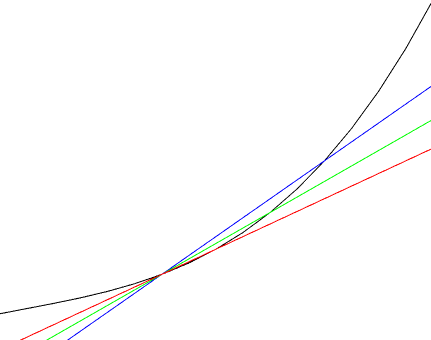
\includegraphics[width = 200pt]{aveROC}
	\caption{The derivative of the function \textit{(black)} at $x$ approximated better when the difference between the two points is $h$\textit{(red)} than whenthe difference is $2h$\textit{(green)} and $3h$\textit{(blue)}}.
	\label{figureNM}
\end{figure}
\\

As $h$ approaches $0$, the average rate of change between the two points approaches the instantaneous rate of change at the point $x=x_k$. Let us write this rate of change as $f'(x_k) = c$, for some constant $c$. Now, this $f'(x_k)$ is the derivative of $f(x)$ at $x=x_k$. Generalizing this, the derivative of $f(x)$ at any point is the function $f'(x)$.
\\

\subsection{Newton's Method}
(\cite{PaulNM})For the Newton's method, we start with an initial approximation $x_0$ to the solution of $f(x) = 0$ where $f'(x) \neq 0$. We do not want a linear approximation that does not have a root as we are looking for one. Linear approximation is the use of the tangent line of the function at a point to approximate the function. This idea is accepted since near the point of tangency, the line is so close to the function. \textit{\textbf{Insert linear approximation graphics here.}}

We then get the line tangent to $f(x)$ at $x = x_0$. Given that the slope at the point $(x_0,f(x_0))$ is the value first derivative $f'(x)$ when $x=x_0$, using the point-slope form of a line
$$\Ra y - f(x_0) = f'(x_0)\mult(x-x_0)$$
$$\Ra y = f(x_0) + f'(x_0)\mult(x-x_0)$$
The next approximation to the solution would be the zero of the tangent line. Let that be $(x_1,0)$. To solve for $x_1$,
$$y = f(x_0) + f'(x_0)\mult(x-x_0)$$
$$\Ra 0 = f(x_0) + f'(x_0)\mult(x_1-x_0)$$
$$\Ra f'(x_0)\mult(x_1-x_0) = -f(x_0)$$
$$\Ra x_1-x_0 = -\frac{f(x_0)}{f'(x_0)}$$
$$\Ra x_1 = x_0 -\frac{f(x_0)}{f'(x_0)}.$$
Likewise,
$$\Ra x_2 = x_1 -\frac{f(x_1)}{f'(x_1)}.$$
\begin{figure}[h]
	\center
	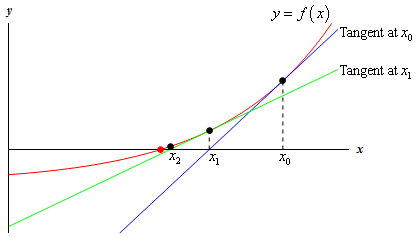
\includegraphics[width = 300pt]{NMGraphics}
	\caption{Graphical representation of Newton's method. (\cite{PaulNM})}
	\label{figureNM}
\end{figure}
Figure \ref{figureNM} portrays what is happening graphically, with the red line being $f(x)$, blue line being the tangent line at $x_0$, and green line being the tangent line at $x_1$. The process will be repeated until we arrive at a good enough approximation, which will be based on our needs. Generalizing this result, if $x_n$ is an approximation to the solution of $f(x) = 0$ and if $f'(x_n)\neq0$, the next approximation would be
$$x_{n+1} = x_n -\frac{f(x_n)}{f'(x_n)}.$$
A way to determine if an approximation is good enough is to compare it to the previous approximation As stated earlier, this process being repeated over and over again is the reason it was called an iterative method.
\\

For example, let $f(x) = x^2 - 1$ and $x_0 = 3$. We first check what we are searching for. So by factoring,
$$x^2 - 1 = 0$$
$$\Ra (x - 1)(x + 1) = 0$$
$$\Ra x - 1 = 0 \quad \textrm{or} \quad x + 1 = 0$$
$$\Ra x = 1 \quad \textrm{or} \quad x = -1.$$
So with this method, we should arive somewhere close at either $x=1$ or $x=-1$.
\\

Now, using the Newton's method, we will have
$$x_{n+1}=x_n - \frac{f(x)}{f'(x)}$$
$$\Ra x_{n+1}=x_n - \frac{x^2-1}{2x}$$
$$\Ra x_{n+1}=\frac{2x_n^2}{2x} - \frac{x^2-1}{2x}$$
$$\Ra x_{n+1}=\frac{x_n^2+1}{2x}.$$
With this,
$$x_1 = \frac{(x_0)^2+1}{2(x_0)} = \frac{(3)^2+1}{2(3)} = \frac{10}{6} = \frac{5}{3}$$
$$x_2 = \frac{(x_1)^2+1}{2(x_1)} = \frac{(5/3)^2+1}{2(5/3)} = \frac{34/9}{10/3} = \frac{17}{15}$$
$$x_3 = \frac{(x_2)^2+1}{2(x_2)} = \frac{(17/15)^2+1}{2(17/15)} = \frac{514/225}{34/15} = \frac{257}{255}$$
$$\Ra x_3 \approx 1.0078.$$
For now, let us be satisfied with this approximation. Depending on the use and need, this approximation may not be considered as far. Usually, people use the stopping criteria
$$\left|f(x_n)\right|<\epsilon\quad\quad\textrm{or}\quad\quad\left| x_{n}-x_{n-1} \right|<\epsilon,$$
where $\epsilon$ is the error the user can tolerate.
\\

\begin{comment}
%Taylor Series
%http://tutorial.math.lamar.edu/Classes/CalcII/TaylorSeries.aspx

Before proceeding to Newton's method, it is ideal that Taylor Series first be introduced for it is crucial in the derivation of the Newton's method. Simply stated, Taylor series is a representation of a differentiable function about a point $x=a$. It should be differentiable for the coefficients are derived from some $n^{th}$ derivative of the function. Mathematically,
\begin{equation}	\label{taylorSer}
	f(x) = \sum_{n=0}^\infty\ds\frac{f^{(n)}(a)}{n!}(x-a)^n,
\end{equation}
where $f^{(n)}$ is the $n^{th}$ derivative of $f$. It has be noted hence that $f(x)$ should be differentiable at any degree. It is also to be noted that $f^{(0)}$ is the function itself.

It is probably safe to say that if we take only a part of the Taylor series expansion, let's say, up to $n=k$, that part will be an approximation of the function $f(x)$. It is necessary to do so for we it is hard for us to solve, if it is even possible, dealing with infinities.

So from the Taylor series, the Newton's method can be derived; however, for the Newton's method, it is enough for the function $f(x)$ is differentiable up to two degrees in some closed interval $[a,b]$ where the second derivative is continuous--it can be written as $f\in C^2[a,b]$.
\end{comment}

\begin{comment}
Using this code in Matlab,
\begin{lstlisting}
x(1) = 10;
i = 1;
while 1
    x(i+1) = x(i) - (func(x(i))/dev(x(i)));
    if(abs(x(i+1)-x(i))<10e-10)
        break;
    end
    i = i + 1;
end
\end{lstlisting}
we would get that $x_1=5.05$, $x_2=2.624010$, $x_3=1.502553$, $x_4=1.084043$, $x_5=1.003258$, and $x_6=1.000005$. $func$ and $dev$ are functions for solving $f(x_n)$ and $f'(x_n)$, respectively.
\end{comment}


\subsection{Ordinary Differential Equations}

A differential equation is an equation involving derivatives of any order. Examples would be: $dy = 3x$, $f''(x) = 4x+6$, and $g^{n} = h(x)$, for some $h$ a function of $x$.
\\

\subsection{Initial-Value Problem}

Before proceeding to the main topic, we need to first understand another concept--the initial value problem. Initial value problem is an ordinary differential equation with a given initial condition, say $f^{(n)}(x_k) = c$. An initial value problem are ODEs to be solved with the initial value to arive at a specific solution.


\subsection{The Continuous Newton's Method}

%From Discrete to Continuous

As stated by Jacobsen in \cite{jacobsen}, in 1870 and 1879, Schr\"oder and Cayley respectively imitated this method for complex polynomials $p(z)$. So with an initial complex value $z_0$, the solution is then found using
\begin{equation}
	z_{n+1} = z_{n} - \ds\frac{p(z_n)}{p'(z_n)},\ z_n \in \mathbb{C}.
\end{equation}

